% \appendix
\section{Networks designed by the agent during training and evaluation}\label{app:networks}

Here we show the best architectures designed by the agent in the three experiments. Figure~\ref{fig:app:networks:training} shows the best architecture per datasets during training (\textit{omniglot}, \textit{vgg\_flower}, and \textit{dtd}). Figure~\ref{fig:app:networks:aircraft} and~\ref{fig:app:networks:cubirds} show the best two architectures during evaluation for \textit{aircraft} and \textit{cu\_birds} respectively. Figure~\ref{fig:app:networks:multibranch} shows the best architectures for the multi-branch experiment. For each architecture we report the early-stop accuracy obtained.

%%%%%%%%%%% Training architectures
\begin{figure}[ht]
\centering
\begin{subfigure}{.33\textwidth}
\begin{center}
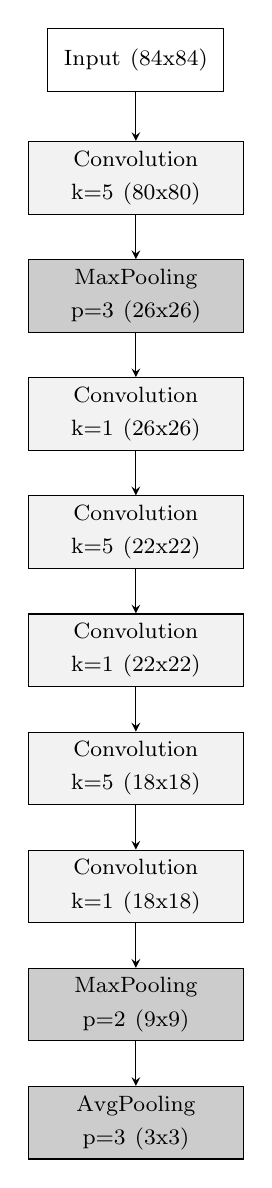
\begin{tikzpicture}

% definitions
\tikzstyle{input} = [rectangle, minimum width=2cm, minimum height=0.8cm, text centered, draw=black, fill=gray!0, text width=2cm]


\tikzstyle{convolution} = [rectangle, minimum width=2cm, minimum height=0.8cm, text centered, draw=black, fill=gray!10, text width=2.5cm]

\tikzstyle{maxpool} = [rectangle, minimum width=2cm, minimum height=0.8cm, text centered, draw=black, fill=gray!40, text width=2.5cm]

\tikzstyle{avgpool} = [rectangle, minimum width=2cm, minimum height=0.8cm, text centered, draw=black, fill=gray!40, text width=2.5cm]

\tikzstyle{concat} = [rectangle, minimum width=2cm, minimum height=0.8cm, text centered, draw=black, fill=gray!80, text width=2.5cm]

\tikzstyle{arrow} = [->,>=stealth]

% the graph
\node (l0) [input] at (0,0) {\footnotesize Input (84x84)};

\node (l1) [convolution, below of=l0, yshift=-0.5cm] {\footnotesize Convolution k=5 (80x80)};

\node (l2) [maxpool, below of=l1, yshift=-0.5cm] {\footnotesize MaxPooling p=3 (26x26)};

\node (l3) [convolution, below of=l2, yshift=-0.5cm] {\footnotesize Convolution k=1 (26x26)};

\node (l4) [convolution, below of=l3, yshift=-0.5cm] {\footnotesize Convolution k=5 (22x22)};

\node (l5) [convolution, below of=l4, yshift=-0.5cm] {\footnotesize Convolution k=1 (22x22)};

\node (l6) [convolution, below of=l5, yshift=-0.5cm] {\footnotesize Convolution k=5 (18x18)};

\node (l7) [convolution, below of=l6, yshift=-0.5cm] {\footnotesize Convolution k=1 (18x18)};

\node (l8) [maxpool, below of=l7, yshift=-0.5cm] {\footnotesize MaxPooling p=2 (9x9)};

\node (l9) [avgpool, below of=l8, yshift=-0.5cm] {\footnotesize AvgPooling p=3 (3x3)};


\draw [arrow] (l0) -- (l1);
\draw [arrow] (l1) -- (l2);
\draw [arrow] (l2) -- (l3);
\draw [arrow] (l3) -- (l4);
\draw [arrow] (l4) -- (l5);
\draw [arrow] (l5) -- (l6);
\draw [arrow] (l6) -- (l7);
\draw [arrow] (l7) -- (l8);
\draw [arrow] (l8) -- (l9);

\end{tikzpicture}
\caption{}
\label{fig:app:networks:training:omniglot}
\end{center}
\end{subfigure}%
\begin{subfigure}{.33\textwidth}
\smallskip
\smallskip
\smallskip
\smallskip
\smallskip
\smallskip
\smallskip
\smallskip
\smallskip
\smallskip
\smallskip
\smallskip
\smallskip
\smallskip
\smallskip
\smallskip
\smallskip
\smallskip
\smallskip
\smallskip
\smallskip
\begin{center}
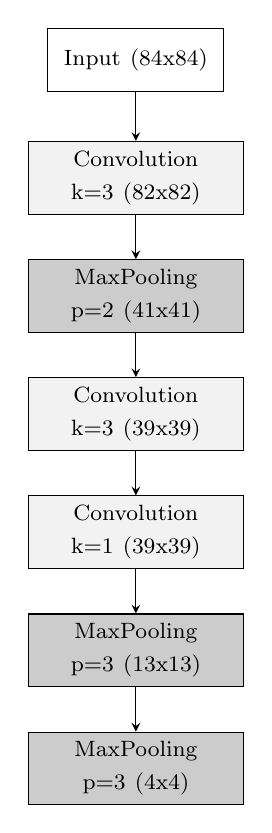
\begin{tikzpicture}

% definitions
\tikzstyle{input} = [rectangle, minimum width=2cm, minimum height=0.8cm, text centered, draw=black, fill=gray!0, text width=2cm]


\tikzstyle{convolution} = [rectangle, minimum width=2cm, minimum height=0.8cm, text centered, draw=black, fill=gray!10, text width=2.5cm]

\tikzstyle{maxpool} = [rectangle, minimum width=2cm, minimum height=0.8cm, text centered, draw=black, fill=gray!40, text width=2.5cm]

\tikzstyle{avgpool} = [rectangle, minimum width=2cm, minimum height=0.8cm, text centered, draw=black, fill=gray!40, text width=2.5cm]

\tikzstyle{concat} = [rectangle, minimum width=2cm, minimum height=0.8cm, text centered, draw=black, fill=gray!80, text width=2.5cm]

\tikzstyle{arrow} = [->,>=stealth]

% the graph
\node (l0) [input] at (0,0) {\footnotesize Input (84x84)};

\node (l1) [convolution, below of=l0, yshift=-0.5cm] {\footnotesize Convolution k=3 (82x82)};

\node (l2) [maxpool, below of=l1, yshift=-0.5cm] {\footnotesize MaxPooling p=2 (41x41)};

\node (l3) [convolution, below of=l2, yshift=-0.5cm] {\footnotesize Convolution k=3 (39x39)};

\node (l4) [convolution, below of=l3, yshift=-0.5cm] {\footnotesize Convolution k=1 (39x39)};

\node (l5) [maxpool, below of=l4, yshift=-0.5cm] {\footnotesize MaxPooling p=3 (13x13)};


\node (l6) [maxpool, below of=l5, yshift=-0.5cm] {\footnotesize MaxPooling p=3 (4x4)};

\draw [arrow] (l0) -- (l1);
\draw [arrow] (l1) -- (l2);
\draw [arrow] (l2) -- (l3);
\draw [arrow] (l3) -- (l4);
\draw [arrow] (l4) -- (l5);
\draw [arrow] (l5) -- (l6);

\end{tikzpicture}
\small
\smallskip
\smallskip
\smallskip
\smallskip
\smallskip
\smallskip
\smallskip
\smallskip
\smallskip
\smallskip
\smallskip
\smallskip
\smallskip
\smallskip
\smallskip
\smallskip
\smallskip
\smallskip
\smallskip
\smallskip
\smallskip
\smallskip
\caption{}
\label{fig:app:networks:training:vggflower}
\end{center}
\end{subfigure}%
\begin{subfigure}{.33\textwidth}
\smallskip
\smallskip
\smallskip
\smallskip
\smallskip
\smallskip
\smallskip
\smallskip
\smallskip
\smallskip
\smallskip
\smallskip
\smallskip
\smallskip
\begin{center}
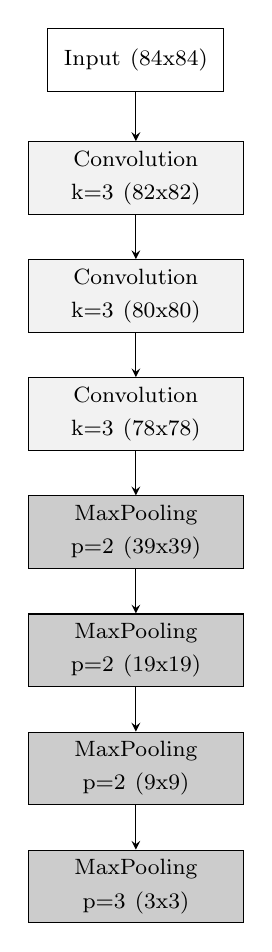
\begin{tikzpicture}

% definitions
\tikzstyle{input} = [rectangle, minimum width=2cm, minimum height=0.8cm, text centered, draw=black, fill=gray!0, text width=2cm]


\tikzstyle{convolution} = [rectangle, minimum width=2cm, minimum height=0.8cm, text centered, draw=black, fill=gray!10, text width=2.5cm]

\tikzstyle{maxpool} = [rectangle, minimum width=2cm, minimum height=0.8cm, text centered, draw=black, fill=gray!40, text width=2.5cm]

\tikzstyle{avgpool} = [rectangle, minimum width=2cm, minimum height=0.8cm, text centered, draw=black, fill=gray!40, text width=2.5cm]

\tikzstyle{concat} = [rectangle, minimum width=2cm, minimum height=0.8cm, text centered, draw=black, fill=gray!80, text width=2.5cm]

\tikzstyle{arrow} = [->,>=stealth]

% the graph
\node (l0) [input] at (0,0) {\footnotesize Input (84x84)};

\node (l1) [convolution, below of=l0, yshift=-0.5cm] {\footnotesize Convolution k=3 (82x82)};

\node (l2) [convolution, below of=l1, yshift=-0.5cm] {\footnotesize Convolution k=3 (80x80)};

\node (l3) [convolution, below of=l2, yshift=-0.5cm] {\footnotesize Convolution k=3 (78x78)};

\node (l4) [maxpool, below of=l3, yshift=-0.5cm] {\footnotesize MaxPooling p=2 (39x39)};

\node (l5) [maxpool, below of=l4, yshift=-0.5cm] {\footnotesize MaxPooling p=2 (19x19)};

\node (l6) [maxpool, below of=l5, yshift=-0.5cm] {\footnotesize MaxPooling p=2 (9x9)};

\node (l7) [maxpool, below of=l6, yshift=-0.5cm] {\footnotesize MaxPooling p=3 (3x3)};


\draw [arrow] (l0) -- (l1);
\draw [arrow] (l1) -- (l2);
\draw [arrow] (l2) -- (l3);
\draw [arrow] (l3) -- (l4);
\draw [arrow] (l4) -- (l5);
\draw [arrow] (l5) -- (l6);
\draw [arrow] (l6) -- (l7);

\end{tikzpicture}
\smallskip
\smallskip
\smallskip
\smallskip
\smallskip
\smallskip
\smallskip
\smallskip
\smallskip
\smallskip
\smallskip
\smallskip
\smallskip
\smallskip
\caption{}
\label{fig:app:networks:training:dtd}
\end{center}
\end{subfigure}
\caption{Best architectures designed for the training datasets. (a) The best architecture for \textit{omniglot}, with early-stop accuracy of 67.11. (b) The best architecture for \textit{vgg\_flower}, with early-stop accuracy of 55.75. (c) The best architecture for \textit{dtd}, with early-stop accuracy of 29.32}
\label{fig:app:networks:training}
\vspace{-0.5cm}
\end{figure}


%%%%%%%%%%%% AIRCRAFT
\begin{figure}[ht]
\centering
\begin{subfigure}{.40\textwidth}
\smallskip
\smallskip
\smallskip
\smallskip
\smallskip
\smallskip
\smallskip
\begin{center}
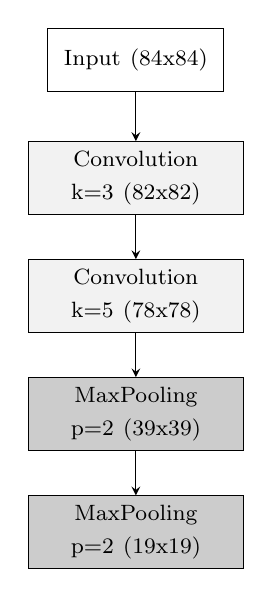
\begin{tikzpicture}

% definitions
\tikzstyle{input} = [rectangle, minimum width=2cm, minimum height=0.8cm, text centered, draw=black, fill=gray!0, text width=2cm]


\tikzstyle{convolution} = [rectangle, minimum width=2cm, minimum height=0.8cm, text centered, draw=black, fill=gray!10, text width=2.5cm]

\tikzstyle{maxpool} = [rectangle, minimum width=2cm, minimum height=0.8cm, text centered, draw=black, fill=gray!40, text width=2.5cm]

\tikzstyle{avgpool} = [rectangle, minimum width=2cm, minimum height=0.8cm, text centered, draw=black, fill=gray!40, text width=2.5cm]

\tikzstyle{concat} = [rectangle, minimum width=2cm, minimum height=0.8cm, text centered, draw=black, fill=gray!80, text width=2.5cm]

\tikzstyle{arrow} = [->,>=stealth]

% the graph
\node (l0) [input] at (0,0) {\footnotesize Input (84x84)};

\node (l1) [convolution, below of=l0, yshift=-0.5cm] {\footnotesize Convolution k=3 (82x82)};

\node (l2) [convolution, below of=l1, yshift=-0.5cm] {\footnotesize Convolution k=5 (78x78)};

\node (l3) [maxpool, below of=l2, yshift=-0.5cm] {\footnotesize MaxPooling p=2 (39x39)};

\node (l4) [maxpool, below of=l3, yshift=-0.5cm] {\footnotesize MaxPooling p=2 (19x19)};


\draw [arrow] (l0) -- (l1);
\draw [arrow] (l1) -- (l2);
\draw [arrow] (l2) -- (l3);
\draw [arrow] (l3) -- (l4);

\end{tikzpicture}
\smallskip
\smallskip
\smallskip
\smallskip
\smallskip
\smallskip
\smallskip
\caption{}
\label{fig:app:networks:aircraft:a}
\end{center}
\end{subfigure}%
\begin{subfigure}{.40\textwidth}
\begin{center}
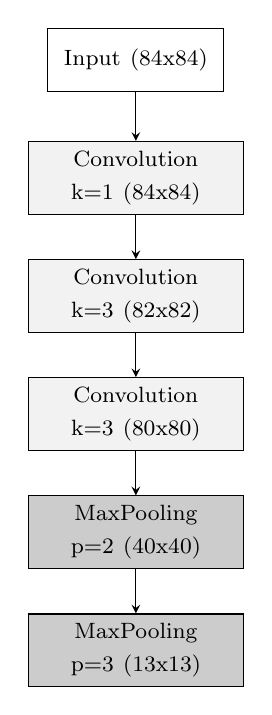
\begin{tikzpicture}

% definitions
\tikzstyle{input} = [rectangle, minimum width=2cm, minimum height=0.8cm, text centered, draw=black, fill=gray!0, text width=2cm]


\tikzstyle{convolution} = [rectangle, minimum width=2cm, minimum height=0.8cm, text centered, draw=black, fill=gray!10, text width=2.5cm]

\tikzstyle{maxpool} = [rectangle, minimum width=2cm, minimum height=0.8cm, text centered, draw=black, fill=gray!40, text width=2.5cm]

\tikzstyle{avgpool} = [rectangle, minimum width=2cm, minimum height=0.8cm, text centered, draw=black, fill=gray!40, text width=2.5cm]

\tikzstyle{concat} = [rectangle, minimum width=2cm, minimum height=0.8cm, text centered, draw=black, fill=gray!80, text width=2.5cm]

\tikzstyle{arrow} = [->,>=stealth]

% the graph
\node (l0) [input] at (0,0) {\footnotesize Input (84x84)};

\node (l1) [convolution, below of=l0, yshift=-0.5cm] {\footnotesize Convolution k=1 (84x84)};

\node (l2) [convolution, below of=l1, yshift=-0.5cm] {\footnotesize Convolution k=3 (82x82)};

\node (l3) [convolution, below of=l2, yshift=-0.5cm] {\footnotesize Convolution k=3 (80x80)};

\node (l4) [maxpool, below of=l3, yshift=-0.5cm] {\footnotesize MaxPooling p=2 (40x40)};

\node (l5) [maxpool, below of=l4, yshift=-0.5cm] {\footnotesize MaxPooling p=3 (13x13)};


\draw [arrow] (l0) -- (l1);
\draw [arrow] (l1) -- (l2);
\draw [arrow] (l2) -- (l3);
\draw [arrow] (l3) -- (l4);
\draw [arrow] (l4) -- (l5);

\end{tikzpicture}
\small
\caption{}
\label{fig:app:networks:aircraft:b}
\end{center}
\end{subfigure}
\caption{Best architectures designed for \textit{aircraft} during evaluation of the policy. (a) The best architecture with early-stop accuracy of 48.22. (b) The second-best architecture with early-stop accuracy of 47.95}
\label{fig:app:networks:aircraft}
\vspace{-0.5cm}
\end{figure}


%%%%%%%%% CU BIRDS

\begin{figure}[ht]
\centering
\begin{subfigure}{.40\textwidth}
\begin{center}
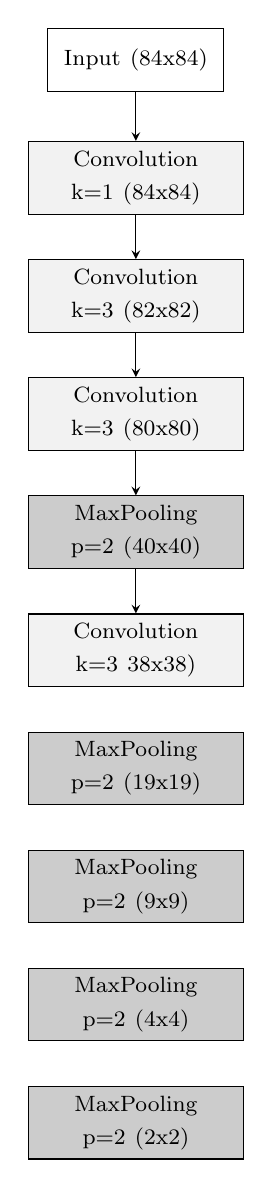
\begin{tikzpicture}

% definitions
\tikzstyle{input} = [rectangle, minimum width=2cm, minimum height=0.8cm, text centered, draw=black, fill=gray!0, text width=2cm]


\tikzstyle{convolution} = [rectangle, minimum width=2cm, minimum height=0.8cm, text centered, draw=black, fill=gray!10, text width=2.5cm]

\tikzstyle{maxpool} = [rectangle, minimum width=2cm, minimum height=0.8cm, text centered, draw=black, fill=gray!40, text width=2.5cm]

\tikzstyle{avgpool} = [rectangle, minimum width=2cm, minimum height=0.8cm, text centered, draw=black, fill=gray!40, text width=2.5cm]

\tikzstyle{concat} = [rectangle, minimum width=2cm, minimum height=0.8cm, text centered, draw=black, fill=gray!80, text width=2.5cm]

\tikzstyle{arrow} = [->,>=stealth]

% the graph
\node (l0) [input] at (0,0) {\footnotesize Input (84x84)};

\node (l1) [convolution, below of=l0, yshift=-0.5cm] {\footnotesize Convolution k=1 (84x84)};

\node (l2) [convolution, below of=l1, yshift=-0.5cm] {\footnotesize Convolution k=3 (82x82)};

\node (l3) [convolution, below of=l2, yshift=-0.5cm] {\footnotesize Convolution k=3 (80x80)};

\node (l4) [maxpool, below of=l3, yshift=-0.5cm] {\footnotesize MaxPooling p=2 (40x40)};

\node (l5) [convolution, below of=l4, yshift=-0.5cm] {\footnotesize Convolution k=3 38x38)};

\node (l6) [maxpool, below of=l5, yshift=-0.5cm] {\footnotesize MaxPooling p=2 (19x19)};

\node (l7) [maxpool, below of=l6, yshift=-0.5cm] {\footnotesize MaxPooling p=2 (9x9)};

\node (l8) [maxpool, below of=l7, yshift=-0.5cm] {\footnotesize MaxPooling p=2 (4x4)};

\node (l9) [maxpool, below of=l8, yshift=-0.5cm] {\footnotesize MaxPooling p=2 (2x2)};

\draw [arrow] (l0) -- (l1);
\draw [arrow] (l1) -- (l2);
\draw [arrow] (l2) -- (l3);
\draw [arrow] (l3) -- (l4);
\draw [arrow] (l4) -- (l5);

\end{tikzpicture}
% \smallskip
% \smallskip
% \smallskip
% \smallskip
% \smallskip
% \smallskip
% \smallskip
% \smallskip
% \smallskip
% \smallskip
% \smallskip
% \smallskip
% \smallskip
% \smallskip
\caption{}
\label{fig:app:networks:cubirds:a}
\end{center}
\end{subfigure}%
\begin{subfigure}{.40\textwidth}
\begin{center}
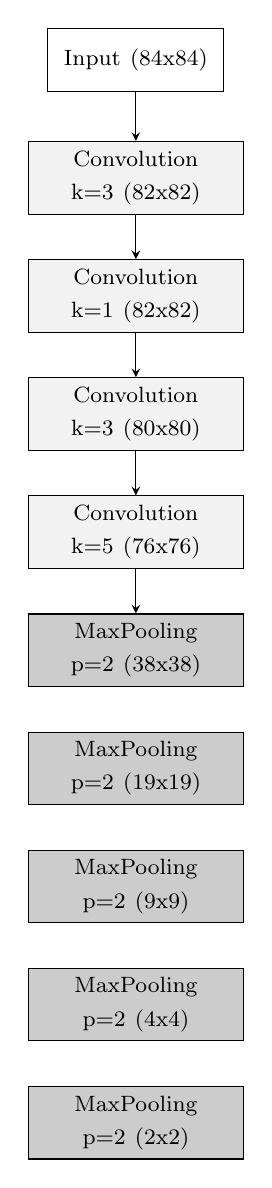
\begin{tikzpicture}

% definitions
\tikzstyle{input} = [rectangle, minimum width=2cm, minimum height=0.8cm, text centered, draw=black, fill=gray!0, text width=2cm]


\tikzstyle{convolution} = [rectangle, minimum width=2cm, minimum height=0.8cm, text centered, draw=black, fill=gray!10, text width=2.5cm]

\tikzstyle{maxpool} = [rectangle, minimum width=2cm, minimum height=0.8cm, text centered, draw=black, fill=gray!40, text width=2.5cm]

\tikzstyle{avgpool} = [rectangle, minimum width=2cm, minimum height=0.8cm, text centered, draw=black, fill=gray!40, text width=2.5cm]

\tikzstyle{concat} = [rectangle, minimum width=2cm, minimum height=0.8cm, text centered, draw=black, fill=gray!80, text width=2.5cm]

\tikzstyle{arrow} = [->,>=stealth]

% the graph
\node (l0) [input] at (0,0) {\footnotesize Input (84x84)};

\node (l1) [convolution, below of=l0, yshift=-0.5cm] {\footnotesize Convolution k=3 (82x82)};

\node (l2) [convolution, below of=l1, yshift=-0.5cm] {\footnotesize Convolution k=1 (82x82)};

\node (l3) [convolution, below of=l2, yshift=-0.5cm] {\footnotesize Convolution k=3 (80x80)};

\node (l4) [convolution, below of=l3, yshift=-0.5cm] {\footnotesize Convolution k=5 (76x76)};

\node (l5) [maxpool, below of=l4, yshift=-0.5cm] {\footnotesize MaxPooling p=2 (38x38)};

\node (l6) [maxpool, below of=l5, yshift=-0.5cm] {\footnotesize MaxPooling p=2 (19x19)};

\node (l7) [maxpool, below of=l6, yshift=-0.5cm] {\footnotesize MaxPooling p=2 (9x9)};

\node (l8) [maxpool, below of=l7, yshift=-0.5cm] {\footnotesize MaxPooling p=2 (4x4)};

\node (l9) [maxpool, below of=l8, yshift=-0.5cm] {\footnotesize MaxPooling p=2 (2x2)};

\draw [arrow] (l0) -- (l1);
\draw [arrow] (l1) -- (l2);
\draw [arrow] (l2) -- (l3);
\draw [arrow] (l3) -- (l4);
\draw [arrow] (l4) -- (l5);

\end{tikzpicture}
\small
\caption{}
\label{fig:app:networks:cubirds:b}
\end{center}
\end{subfigure}
\caption{Best architectures designed for \textit{cu\_birds} during evaluation of the policy. (a) The best architecture with early-stop accuracy of 19.22. (b) The second-best architecture with early-stop accuracy of 19.06}
\label{fig:app:networks:cubirds}
\vspace{-0.5cm}
\end{figure}

%%%%%%%%%%%%%% multibranch

\begin{figure}[ht]
\centering
\begin{subfigure}{.40\textwidth}
\begin{center}
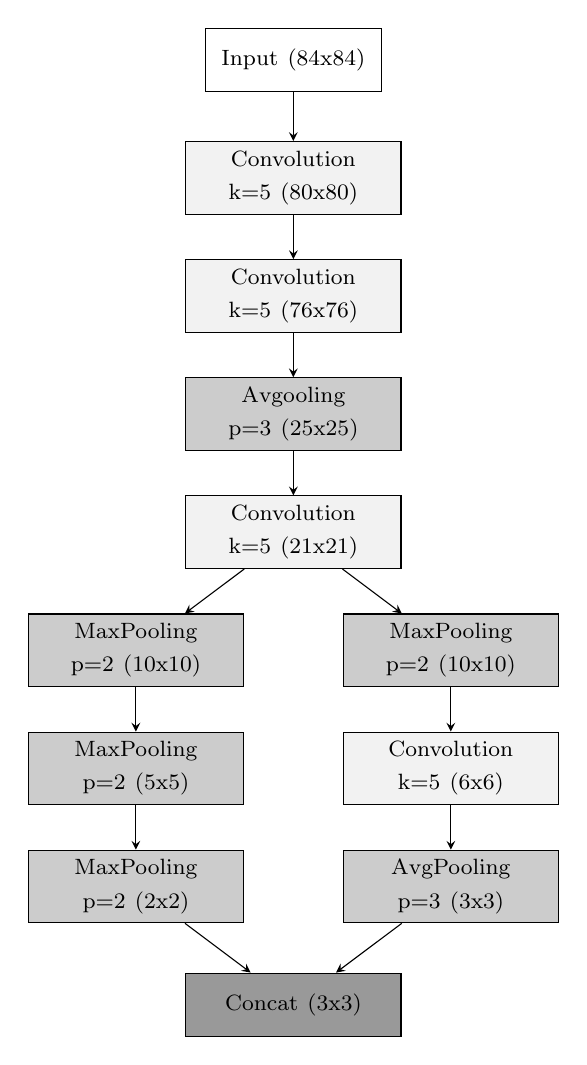
\begin{tikzpicture}

% definitions
\tikzstyle{input} = [rectangle, minimum width=2cm, minimum height=0.8cm, text centered, draw=black, fill=gray!0, text width=2cm]


\tikzstyle{convolution} = [rectangle, minimum width=2cm, minimum height=0.8cm, text centered, draw=black, fill=gray!10, text width=2.5cm]

\tikzstyle{maxpool} = [rectangle, minimum width=2cm, minimum height=0.8cm, text centered, draw=black, fill=gray!40, text width=2.5cm]

\tikzstyle{avgpool} = [rectangle, minimum width=2cm, minimum height=0.8cm, text centered, draw=black, fill=gray!40, text width=2.5cm]

\tikzstyle{concat} = [rectangle, minimum width=2cm, minimum height=0.8cm, text centered, draw=black, fill=gray!80, text width=2.5cm]

\tikzstyle{arrow} = [->,>=stealth]

% the graph
\node (l0) [input] at (0,0) {\footnotesize Input (84x84)};

\node (l1) [convolution, below of=l0, yshift=-0.5cm] {\footnotesize Convolution k=5 (80x80)};

\node (l2) [convolution, below of=l1, yshift=-0.5cm] {\footnotesize Convolution k=5 (76x76)};

\node (l3) [avgpool, below of=l2, yshift=-0.5cm] {\footnotesize Avgooling p=3 (25x25)};

\node (l4) [convolution, below of=l3, yshift=-0.5cm] {\footnotesize Convolution k=5 (21x21)};

\node (l5) [maxpool, below of=l4, yshift=-0.5cm, xshift=-2cm] {\footnotesize MaxPooling p=2 (10x10)};

\node (l6) [maxpool, below of=l4, yshift=-0.5cm, xshift=2cm] {\footnotesize MaxPooling p=2 (10x10)};

\node (l7) [maxpool, below of=l5, yshift=-0.5cm] {\footnotesize MaxPooling p=2 (5x5)};

\node (l8) [convolution, below of=l6, yshift=-0.5cm] {\footnotesize Convolution k=5 (6x6)};

\node (l9) [maxpool, below of=l7, yshift=-0.5cm] {\footnotesize MaxPooling p=2 (2x2)};

\node (l10) [avgpool, below of=l8, yshift=-0.5cm] {\footnotesize AvgPooling p=3 (3x3)};

\node (l11) [concat, below of=l10, yshift=-0.5cm, xshift=-2cm] {\footnotesize Concat (3x3)};


\draw [arrow] (l0) -- (l1);
\draw [arrow] (l1) -- (l2);
\draw [arrow] (l2) -- (l3);
\draw [arrow] (l3) -- (l4);
\draw [arrow] (l4) -- (l5);
\draw [arrow] (l4) -- (l6);
\draw [arrow] (l5) -- (l7);
\draw [arrow] (l6) -- (l8);
\draw [arrow] (l7) -- (l9);
\draw [arrow] (l8) -- (l10);
\draw [arrow] (l9) -- (l11);
\draw [arrow] (l10) -- (l11);

\end{tikzpicture}
\caption{}
\label{fig:app:networks:multibranch:a}
\end{center}
\end{subfigure}%
\begin{subfigure}{.40\textwidth}
\begin{center}
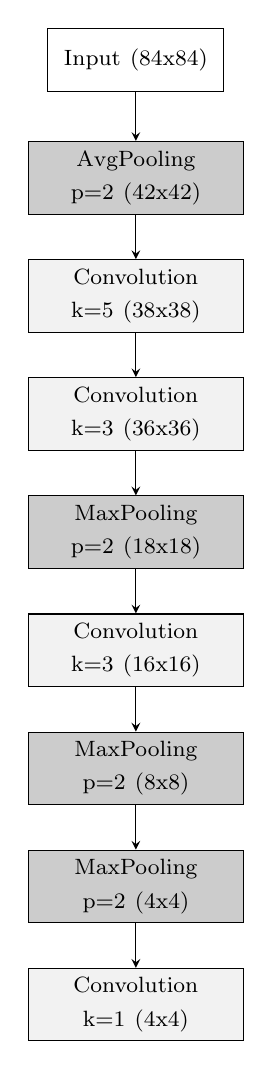
\begin{tikzpicture}

% definitions
\tikzstyle{input} = [rectangle, minimum width=2cm, minimum height=0.8cm, text centered, draw=black, fill=gray!0, text width=2cm]


\tikzstyle{convolution} = [rectangle, minimum width=2cm, minimum height=0.8cm, text centered, draw=black, fill=gray!10, text width=2.5cm]

\tikzstyle{maxpool} = [rectangle, minimum width=2cm, minimum height=0.8cm, text centered, draw=black, fill=gray!40, text width=2.5cm]

\tikzstyle{avgpool} = [rectangle, minimum width=2cm, minimum height=0.8cm, text centered, draw=black, fill=gray!40, text width=2.5cm]

\tikzstyle{concat} = [rectangle, minimum width=2cm, minimum height=0.8cm, text centered, draw=black, fill=gray!80, text width=2.5cm]

\tikzstyle{arrow} = [->,>=stealth]

% the graph
\node (l0) [input] at (0,0) {\footnotesize Input (84x84)};

\node (l1) [avgpool, below of=l0, yshift=-0.5cm] {\footnotesize AvgPooling p=2 (42x42)};

\node (l2) [convolution, below of=l1, yshift=-0.5cm] {\footnotesize Convolution k=5 (38x38)};

\node (l3) [convolution, below of=l2, yshift=-0.5cm] {\footnotesize Convolution k=3 (36x36)};

\node (l4) [maxpool, below of=l3, yshift=-0.5cm] {\footnotesize MaxPooling p=2 (18x18)};

\node (l5) [convolution, below of=l4, yshift=-0.5cm] {\footnotesize Convolution k=3 (16x16)};

\node (l6) [maxpool, below of=l5, yshift=-0.5cm] {\footnotesize MaxPooling p=2 (8x8)};

\node (l7) [maxpool, below of=l6, yshift=-0.5cm] {\footnotesize MaxPooling p=2 (4x4)};

\node (l8) [convolution, below of=l7, yshift=-0.5cm] {\footnotesize Convolution k=1 (4x4)};

\draw [arrow] (l0) -- (l1);
\draw [arrow] (l1) -- (l2);
\draw [arrow] (l2) -- (l3);
\draw [arrow] (l3) -- (l4);
\draw [arrow] (l4) -- (l5);
\draw [arrow] (l5) -- (l6);
\draw [arrow] (l6) -- (l7);
\draw [arrow] (l7) -- (l8);

\end{tikzpicture}
\small
\caption{}
\label{fig:app:networks:multibranch:b}
\end{center}
\end{subfigure}
\caption{Best architectures designed for during the experiment in a multi-branch search space. (a) The best architecture when $\sigma=0.0$, with early-stop accuracy of 66.10. (b) The best architecture when $\sigma=0.1$, with early-stop accuracy of 66.45}
\label{fig:app:networks:multibranch}
\vspace{-0.5cm}
\end{figure}
